\documentclass[12pt,a4paper]{article}

\usepackage[margin=1in]{geometry}
\usepackage{graphicx}
\usepackage{booktabs}
\usepackage{hyperref}
\usepackage{float}
\usepackage{caption}
\usepackage{subcaption}
\usepackage{amsmath}
\usepackage{setspace}
\usepackage{fancyhdr}

\graphicspath{{./}{../screenshots/}}
\hypersetup{colorlinks=true, linkcolor=blue, citecolor=blue, urlcolor=blue}
\pagestyle{fancy}
\fancyhf{}
\rhead{Breast Cancer Classification with ANN}
\lhead{B.Tech AI Mini Project}
\cfoot{\thepage}
\onehalfspacing

\title{
  \vspace{-1cm}
  {\LARGE\textbf{Breast Cancer Classification using\\[0.2cm]
  Artificial Neural Networks}}\\[0.8cm]
  {\large B.Tech Artificial Intelligence -- Mini Project Report}
}
\author{Student Name\\Department of Artificial Intelligence}
\date{\today}

\begin{document}
\maketitle
\begin{abstract}
This report presents a beginner-friendly artificial neural network (ANN) for
binary classification of breast tumors as malignant or benign using the
Breast Cancer Wisconsin dataset. Features are standardized, the model is trained
with the Adam optimizer, and performance is evaluated using accuracy, loss curves,
a confusion matrix, and a classification report. A simple predictive system
returns the diagnosis with class probabilities and confidence.
\end{abstract}

\tableofcontents
\newpage

\section{Introduction}
Breast cancer diagnosis from clinical measurements is a classic machine-learning
problem. In this project we build a compact feed-forward neural network that
maps 30 numeric tumor features to one of two classes:
\textbf{0 = Malignant} and \textbf{1 = Benign}. The implementation uses
TensorFlow/Keras and scikit-learn, and is designed to be easy for beginners to
follow end-to-end.

\section{Dataset}
We use the Breast Cancer Wisconsin (Diagnostic) dataset available in
scikit-learn~\cite{sklearn}. It contains 569 samples and 30 real-valued features
describing cell nuclei characteristics derived from digitized images of fine
needle aspirates.

\begin{figure}[H]
  \centering
  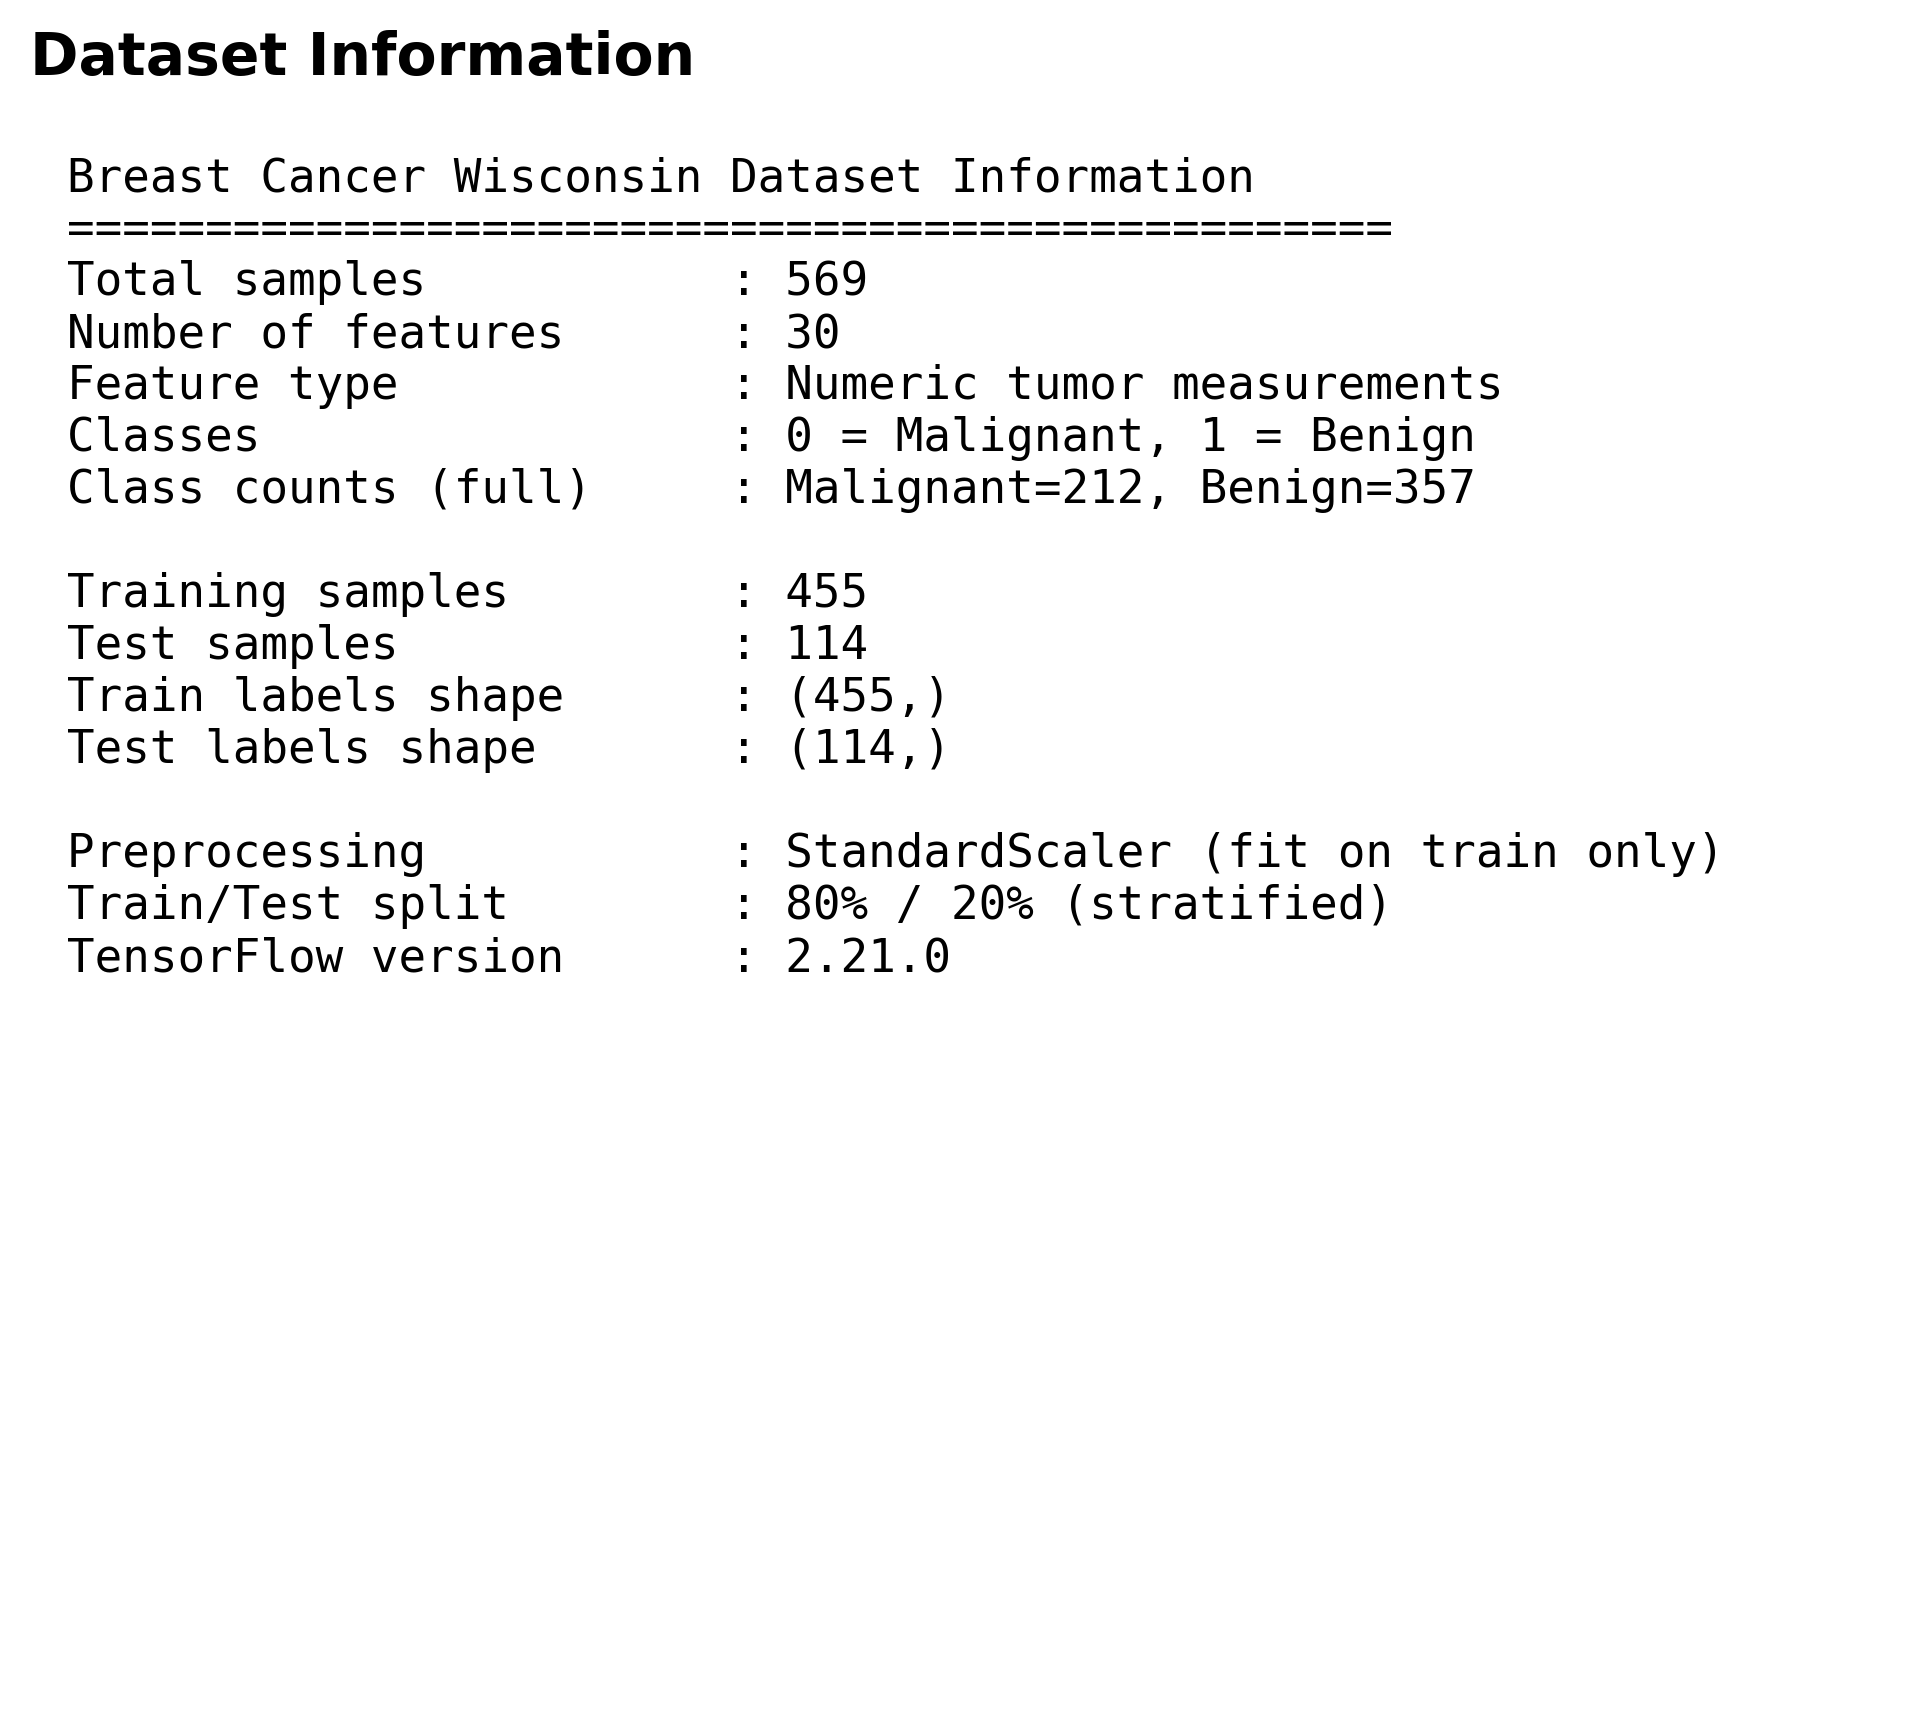
\includegraphics[width=0.95\textwidth]{01_dataset_info.png}
  \caption{Dataset information summary generated by the build pipeline.}
\end{figure}

\begin{figure}[H]
  \centering
  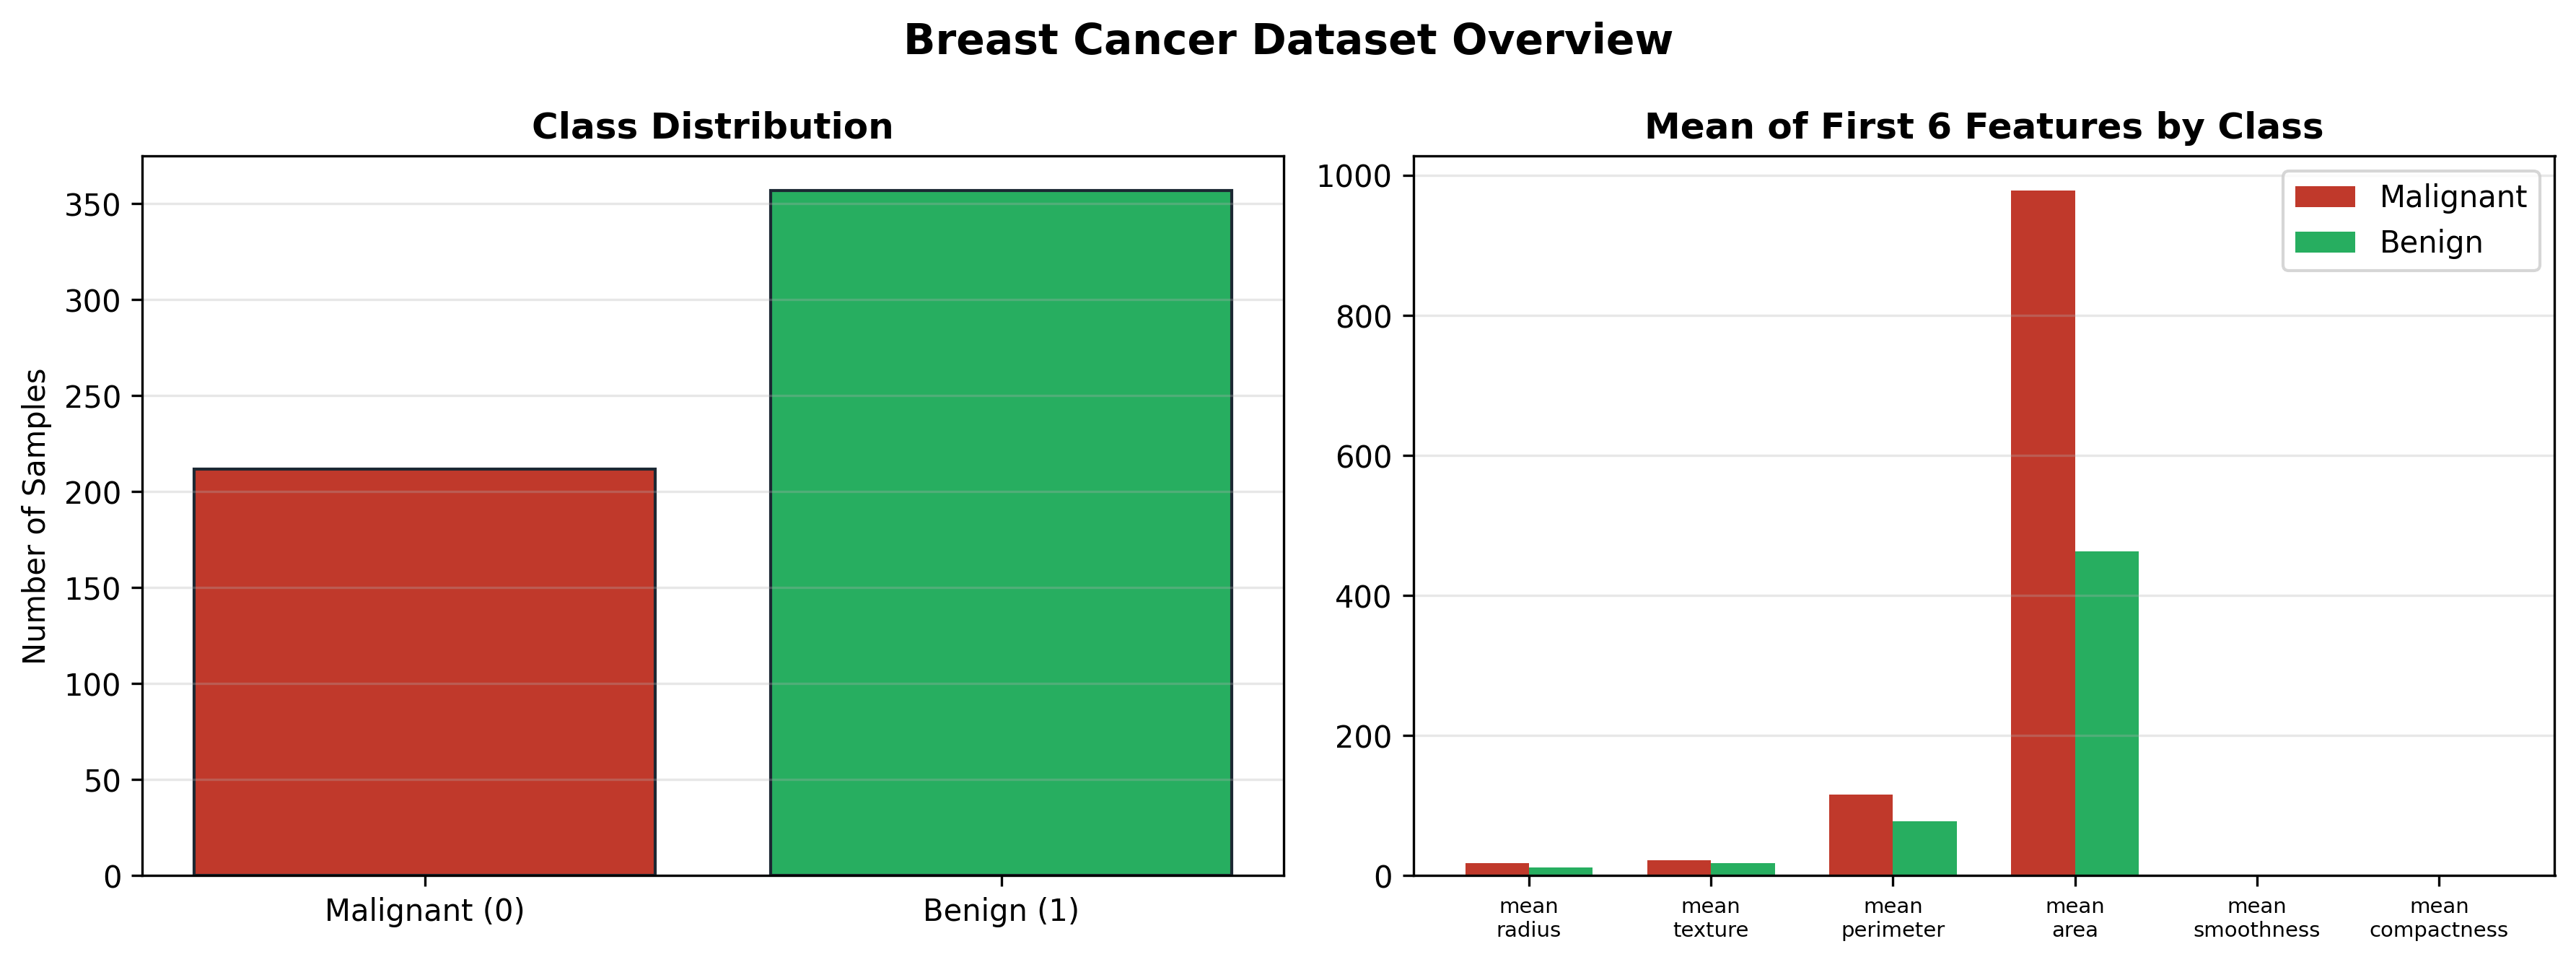
\includegraphics[width=0.95\textwidth]{02_dataset_overview.png}
  \caption{Class distribution and mean feature comparison for selected attributes.}
\end{figure}

\section{Methodology}
\subsection{Preprocessing}
Data are split into training (80\%) and test (20\%) sets with stratification to
preserve class balance. Features are scaled with \texttt{StandardScaler} fitted
only on the training set to avoid data leakage.

\subsection{Model Architecture}
The network is a sequential ANN:
\begin{itemize}
  \item Input layer: 30 features
  \item Hidden layer: 20 neurons with ReLU activation
  \item Output layer: 2 neurons with Softmax activation
\end{itemize}
The model is compiled with the Adam optimizer and sparse categorical
cross-entropy loss.

\begin{figure}[H]
  \centering
  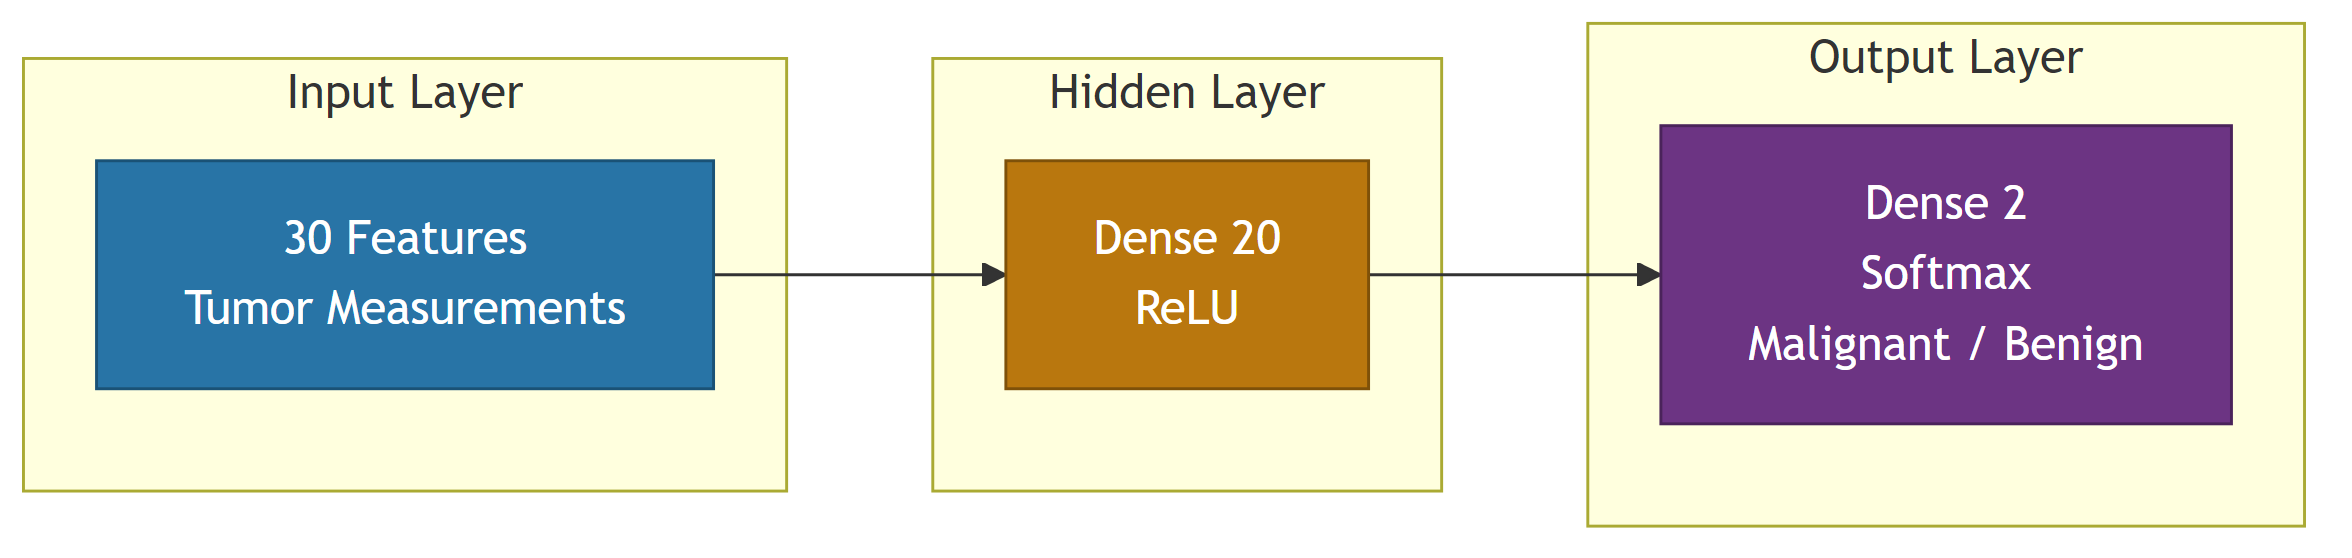
\includegraphics[width=0.85\textwidth]{12_architecture.png}
  \caption{ANN architecture used for breast cancer classification.}
\end{figure}

\begin{figure}[H]
  \centering
  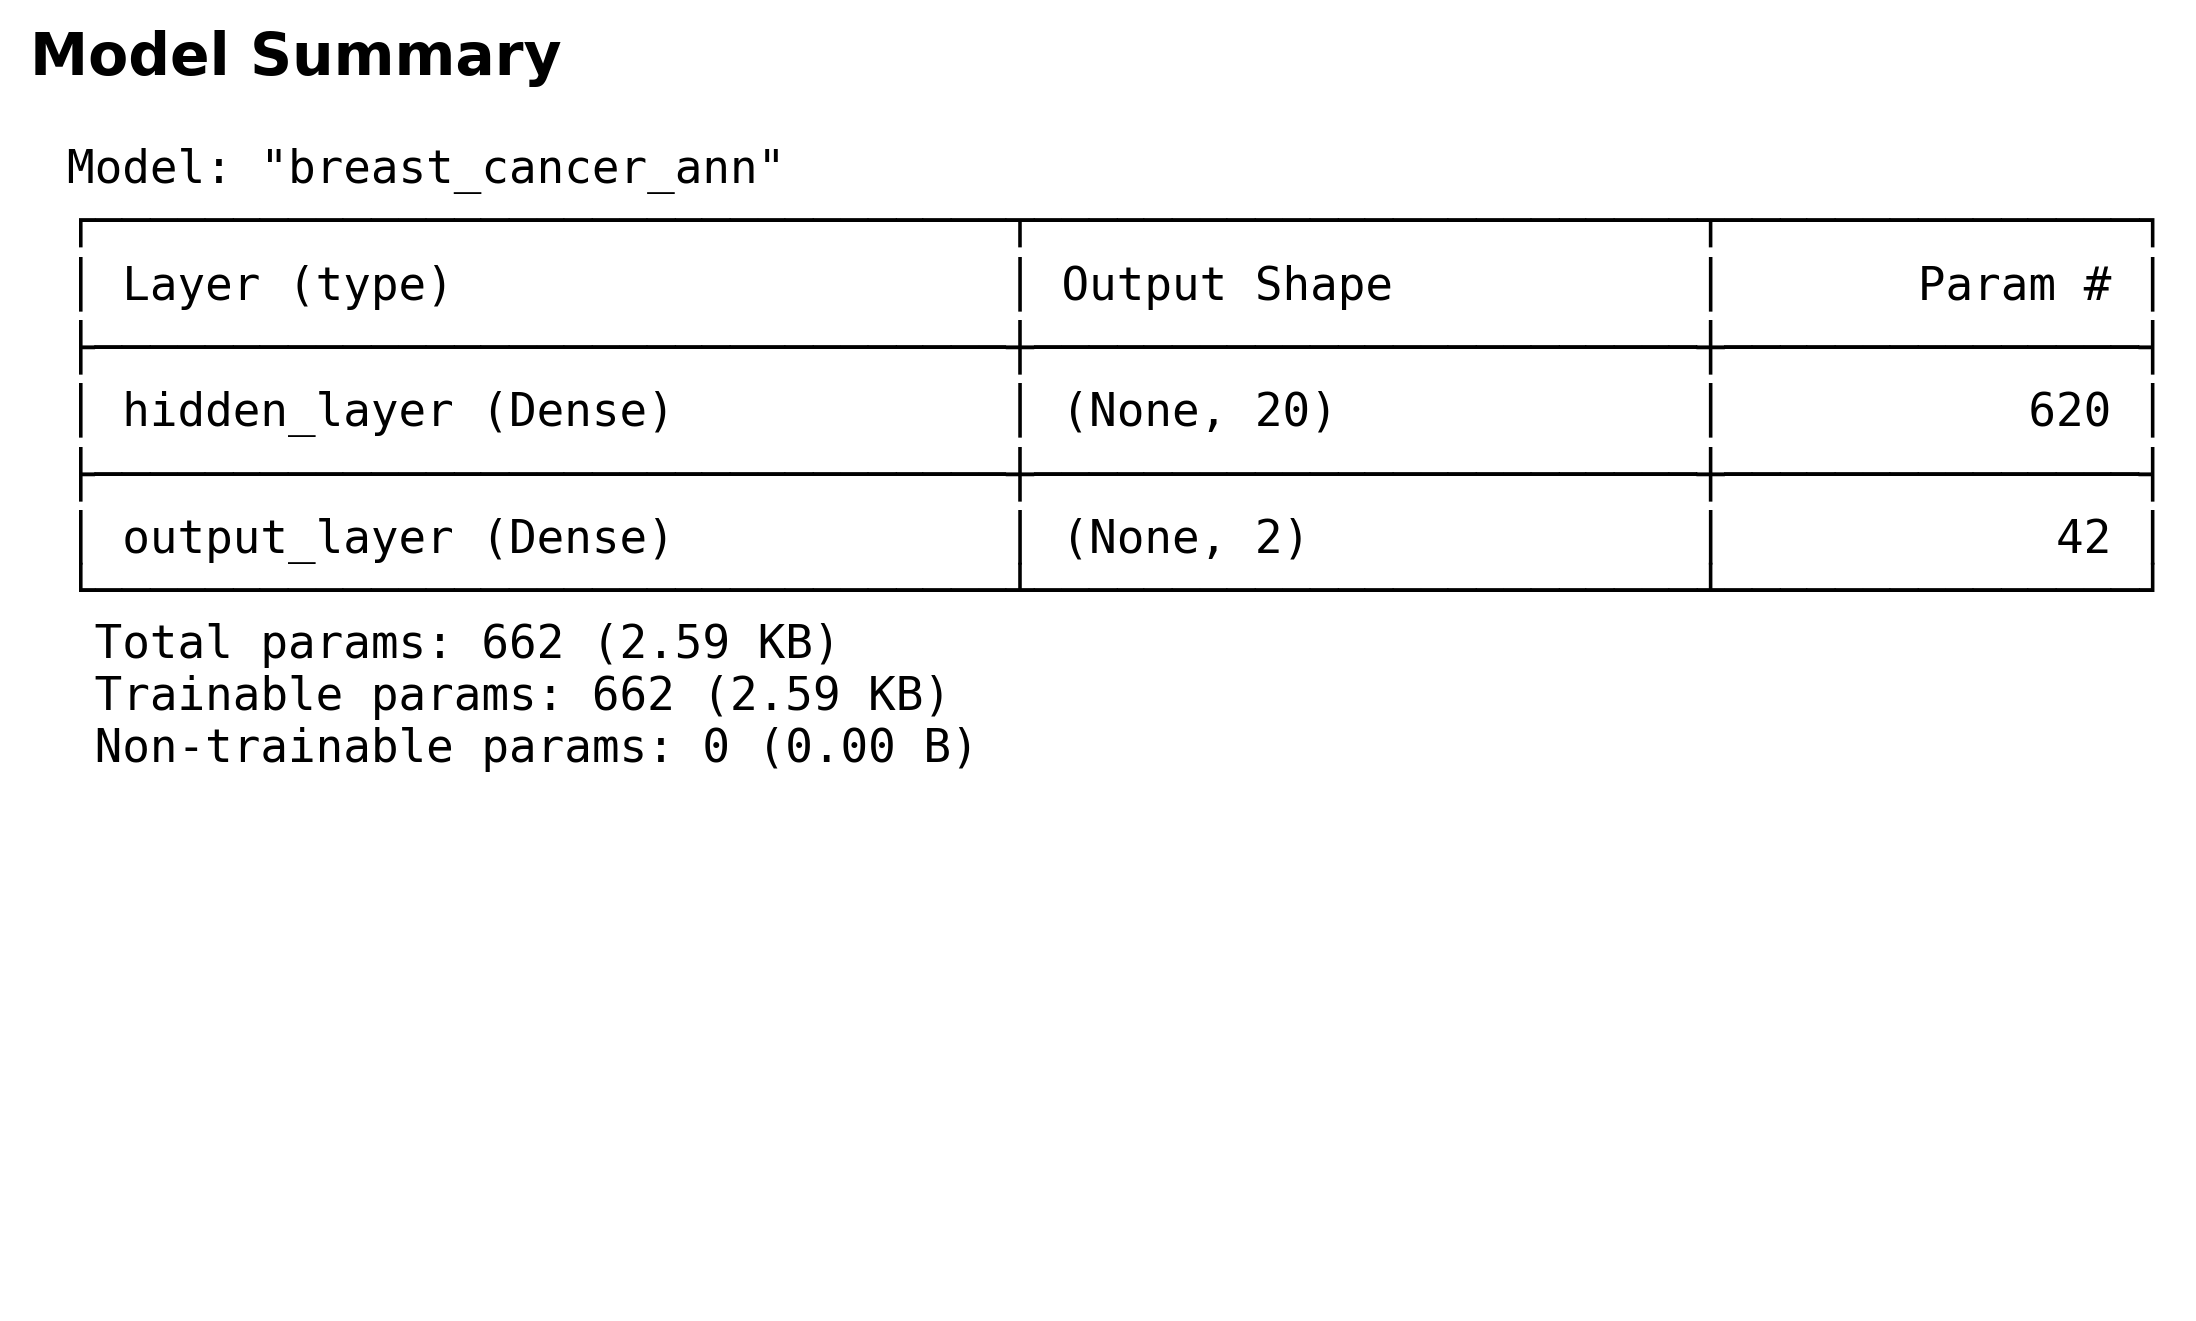
\includegraphics[width=0.85\textwidth]{03_model_summary.png}
  \caption{Keras model summary showing layer shapes and parameter counts.}
\end{figure}

\section{Training}
The model is trained for 10 epochs with a 10\% validation split from the
training data. Accuracy and loss are monitored on both training and validation
sets.

\begin{figure}[H]
  \centering
  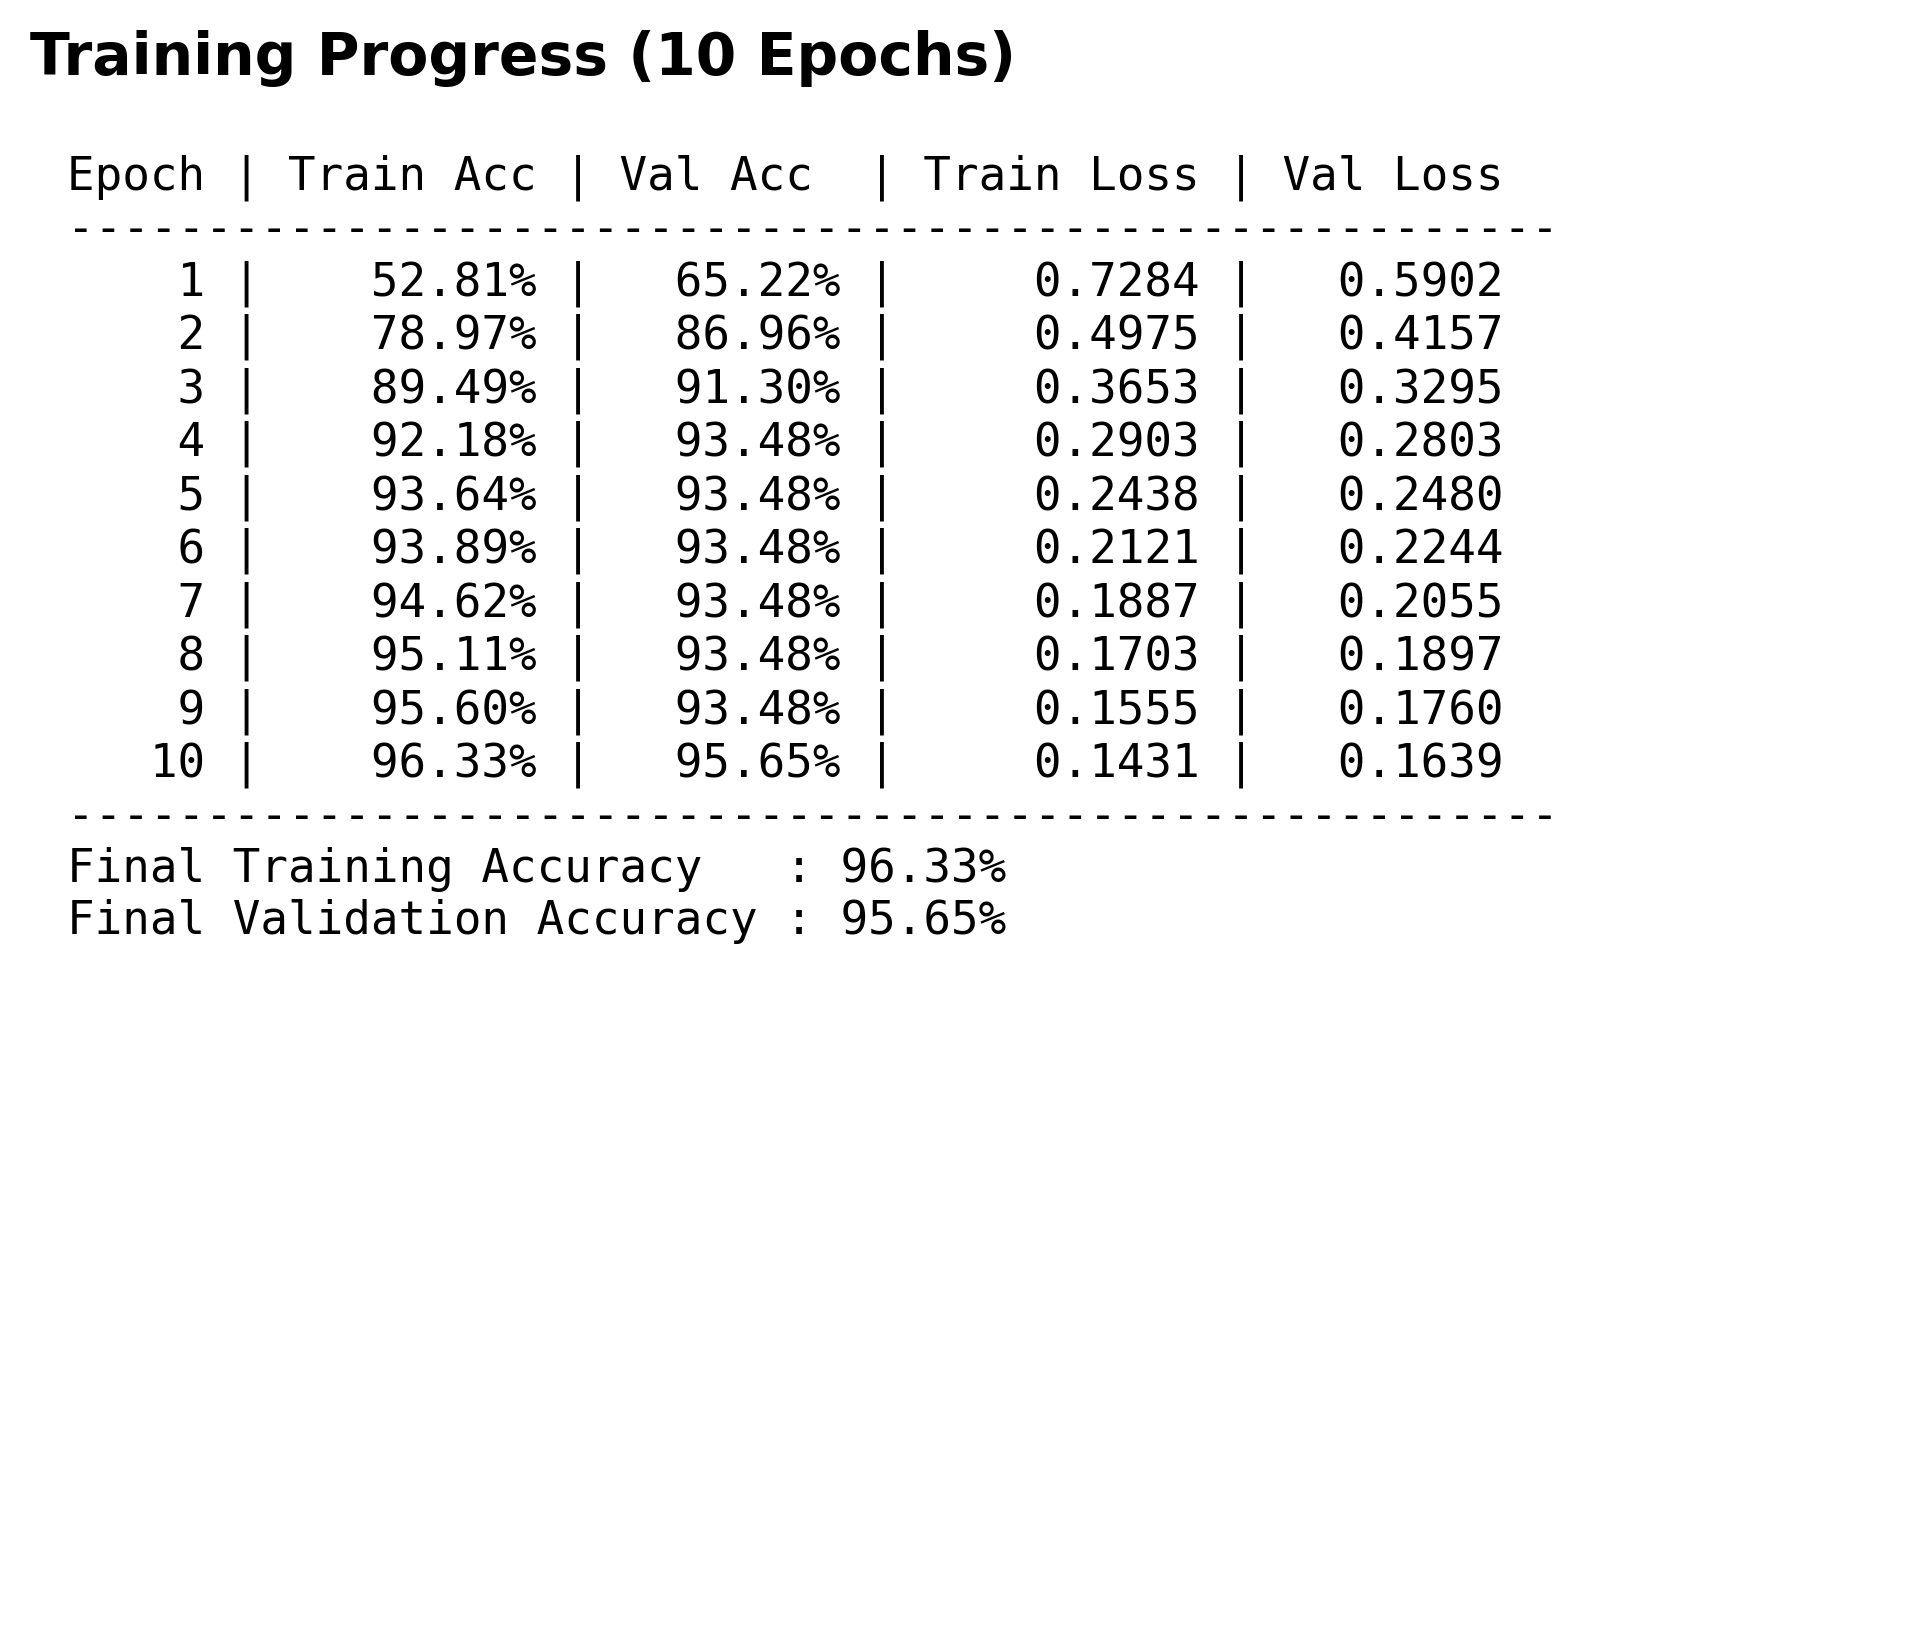
\includegraphics[width=0.9\textwidth]{04_training_progress.png}
  \caption{Per-epoch training and validation metrics.}
\end{figure}

\begin{figure}[H]
  \centering
  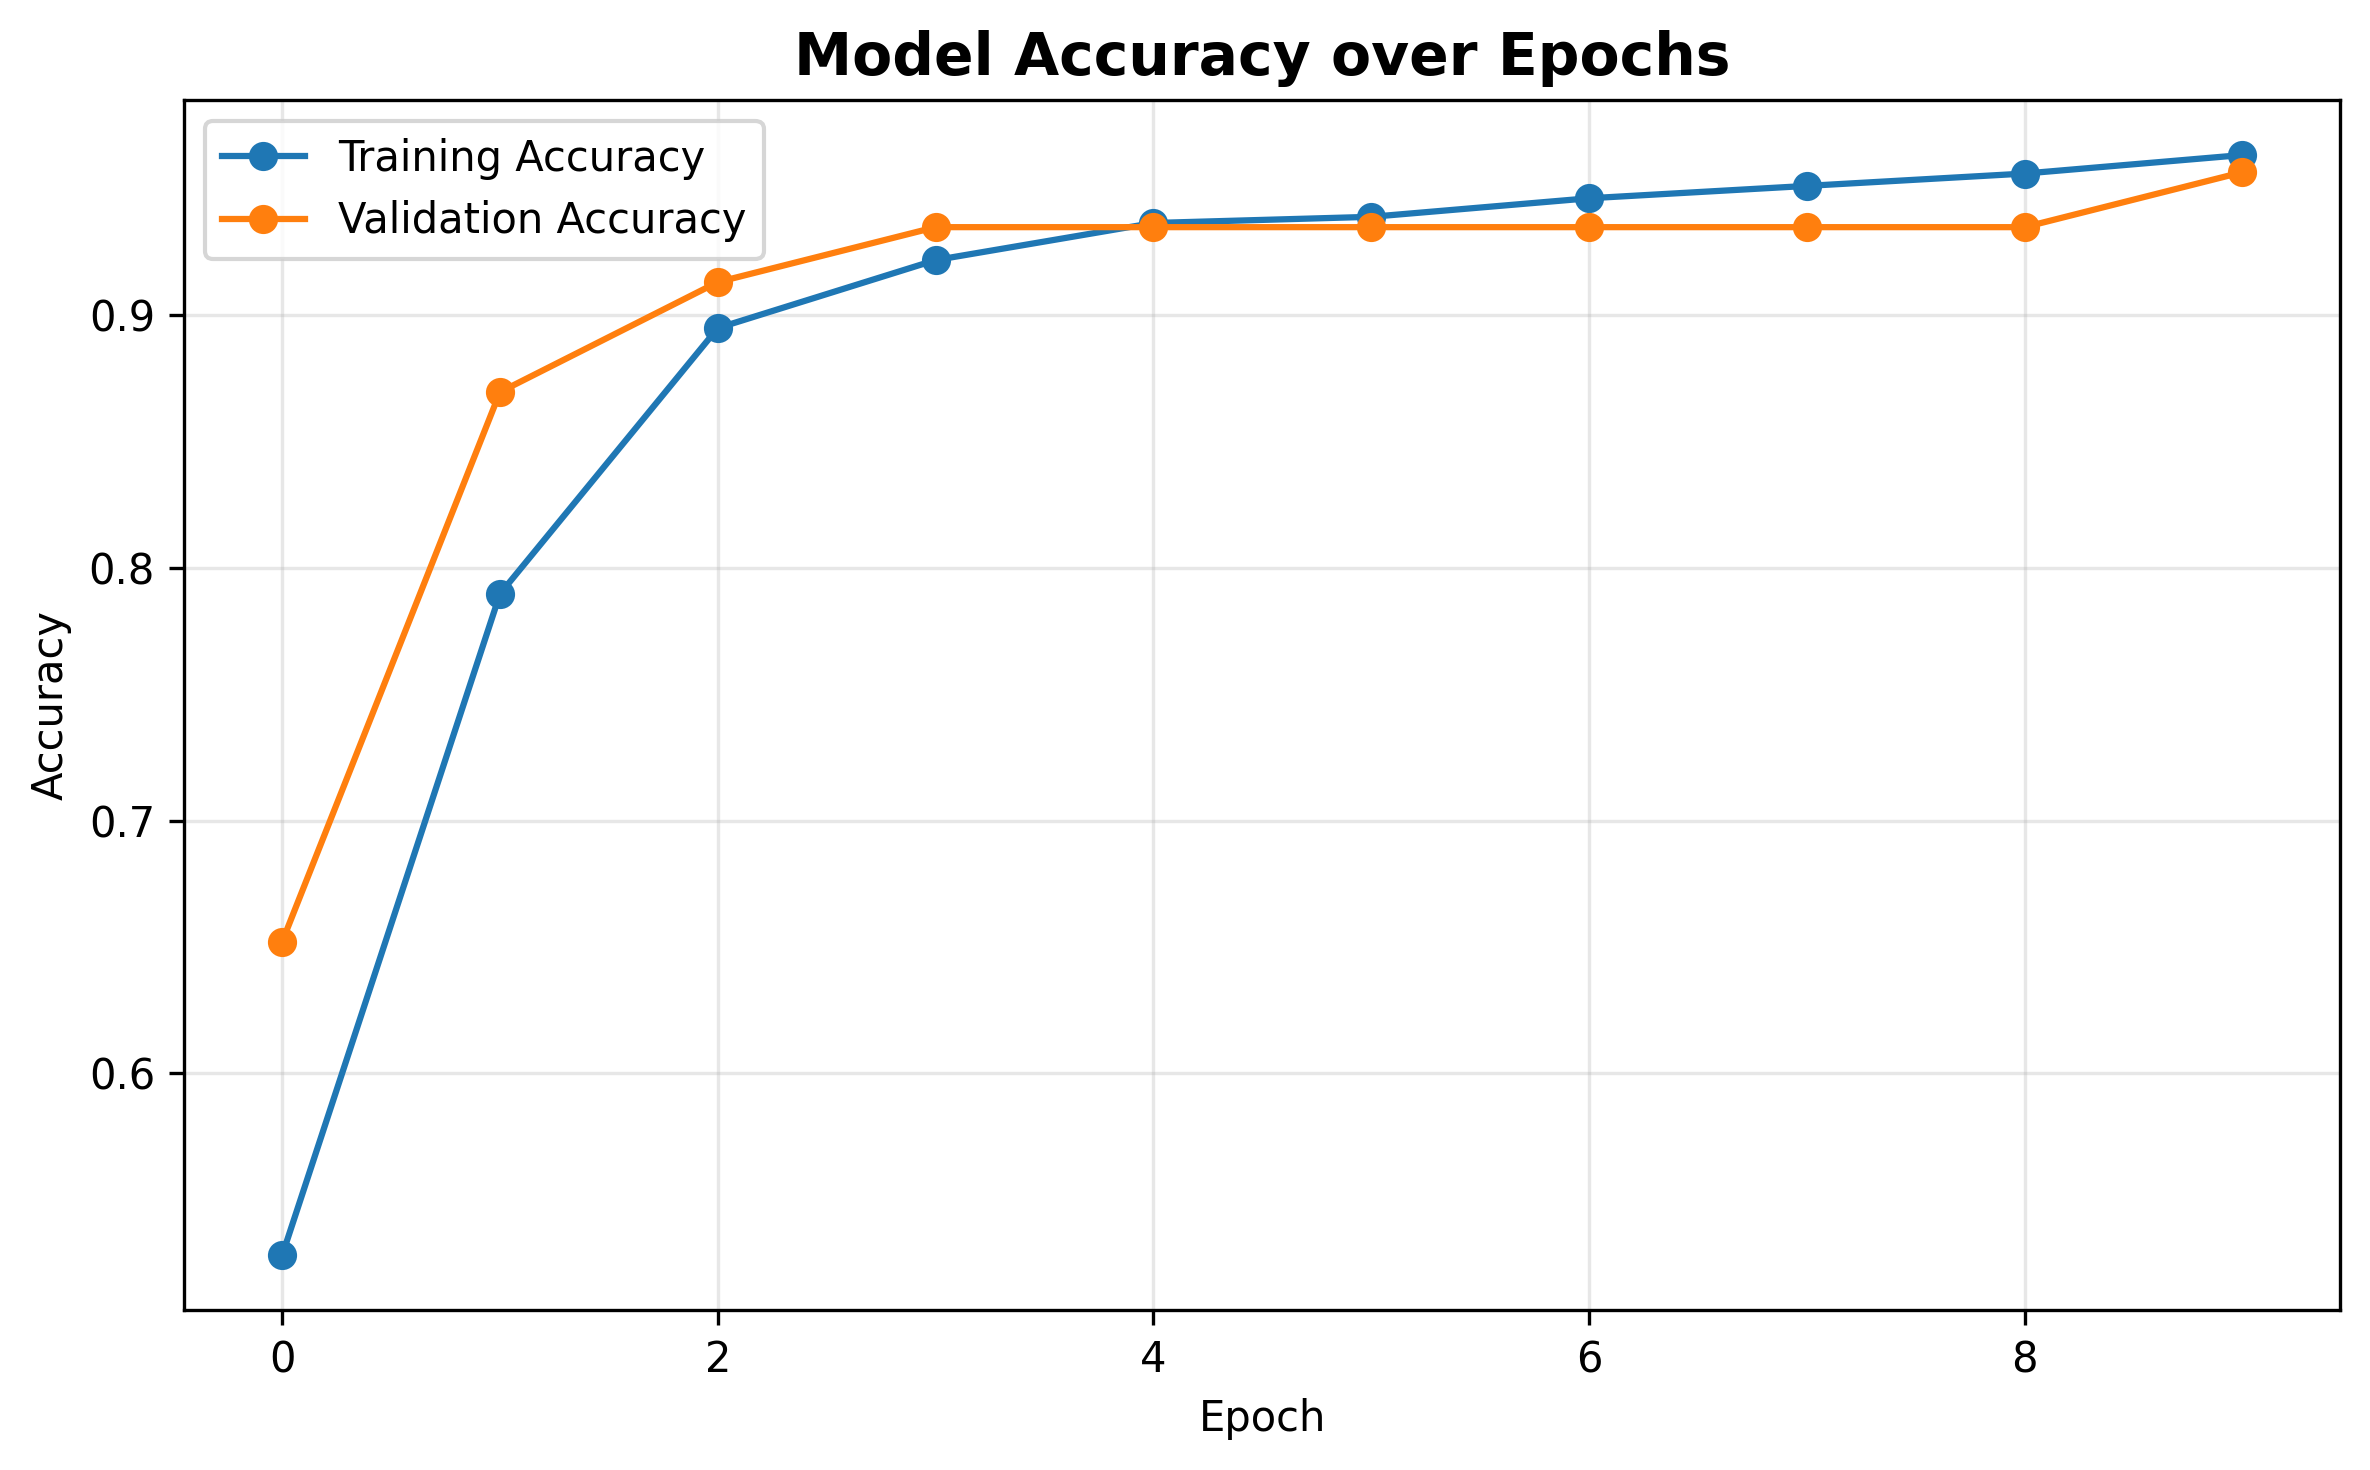
\includegraphics[width=0.85\textwidth]{05_accuracy_curve.png}
  \caption{Training and validation accuracy over epochs.}
\end{figure}

\begin{figure}[H]
  \centering
  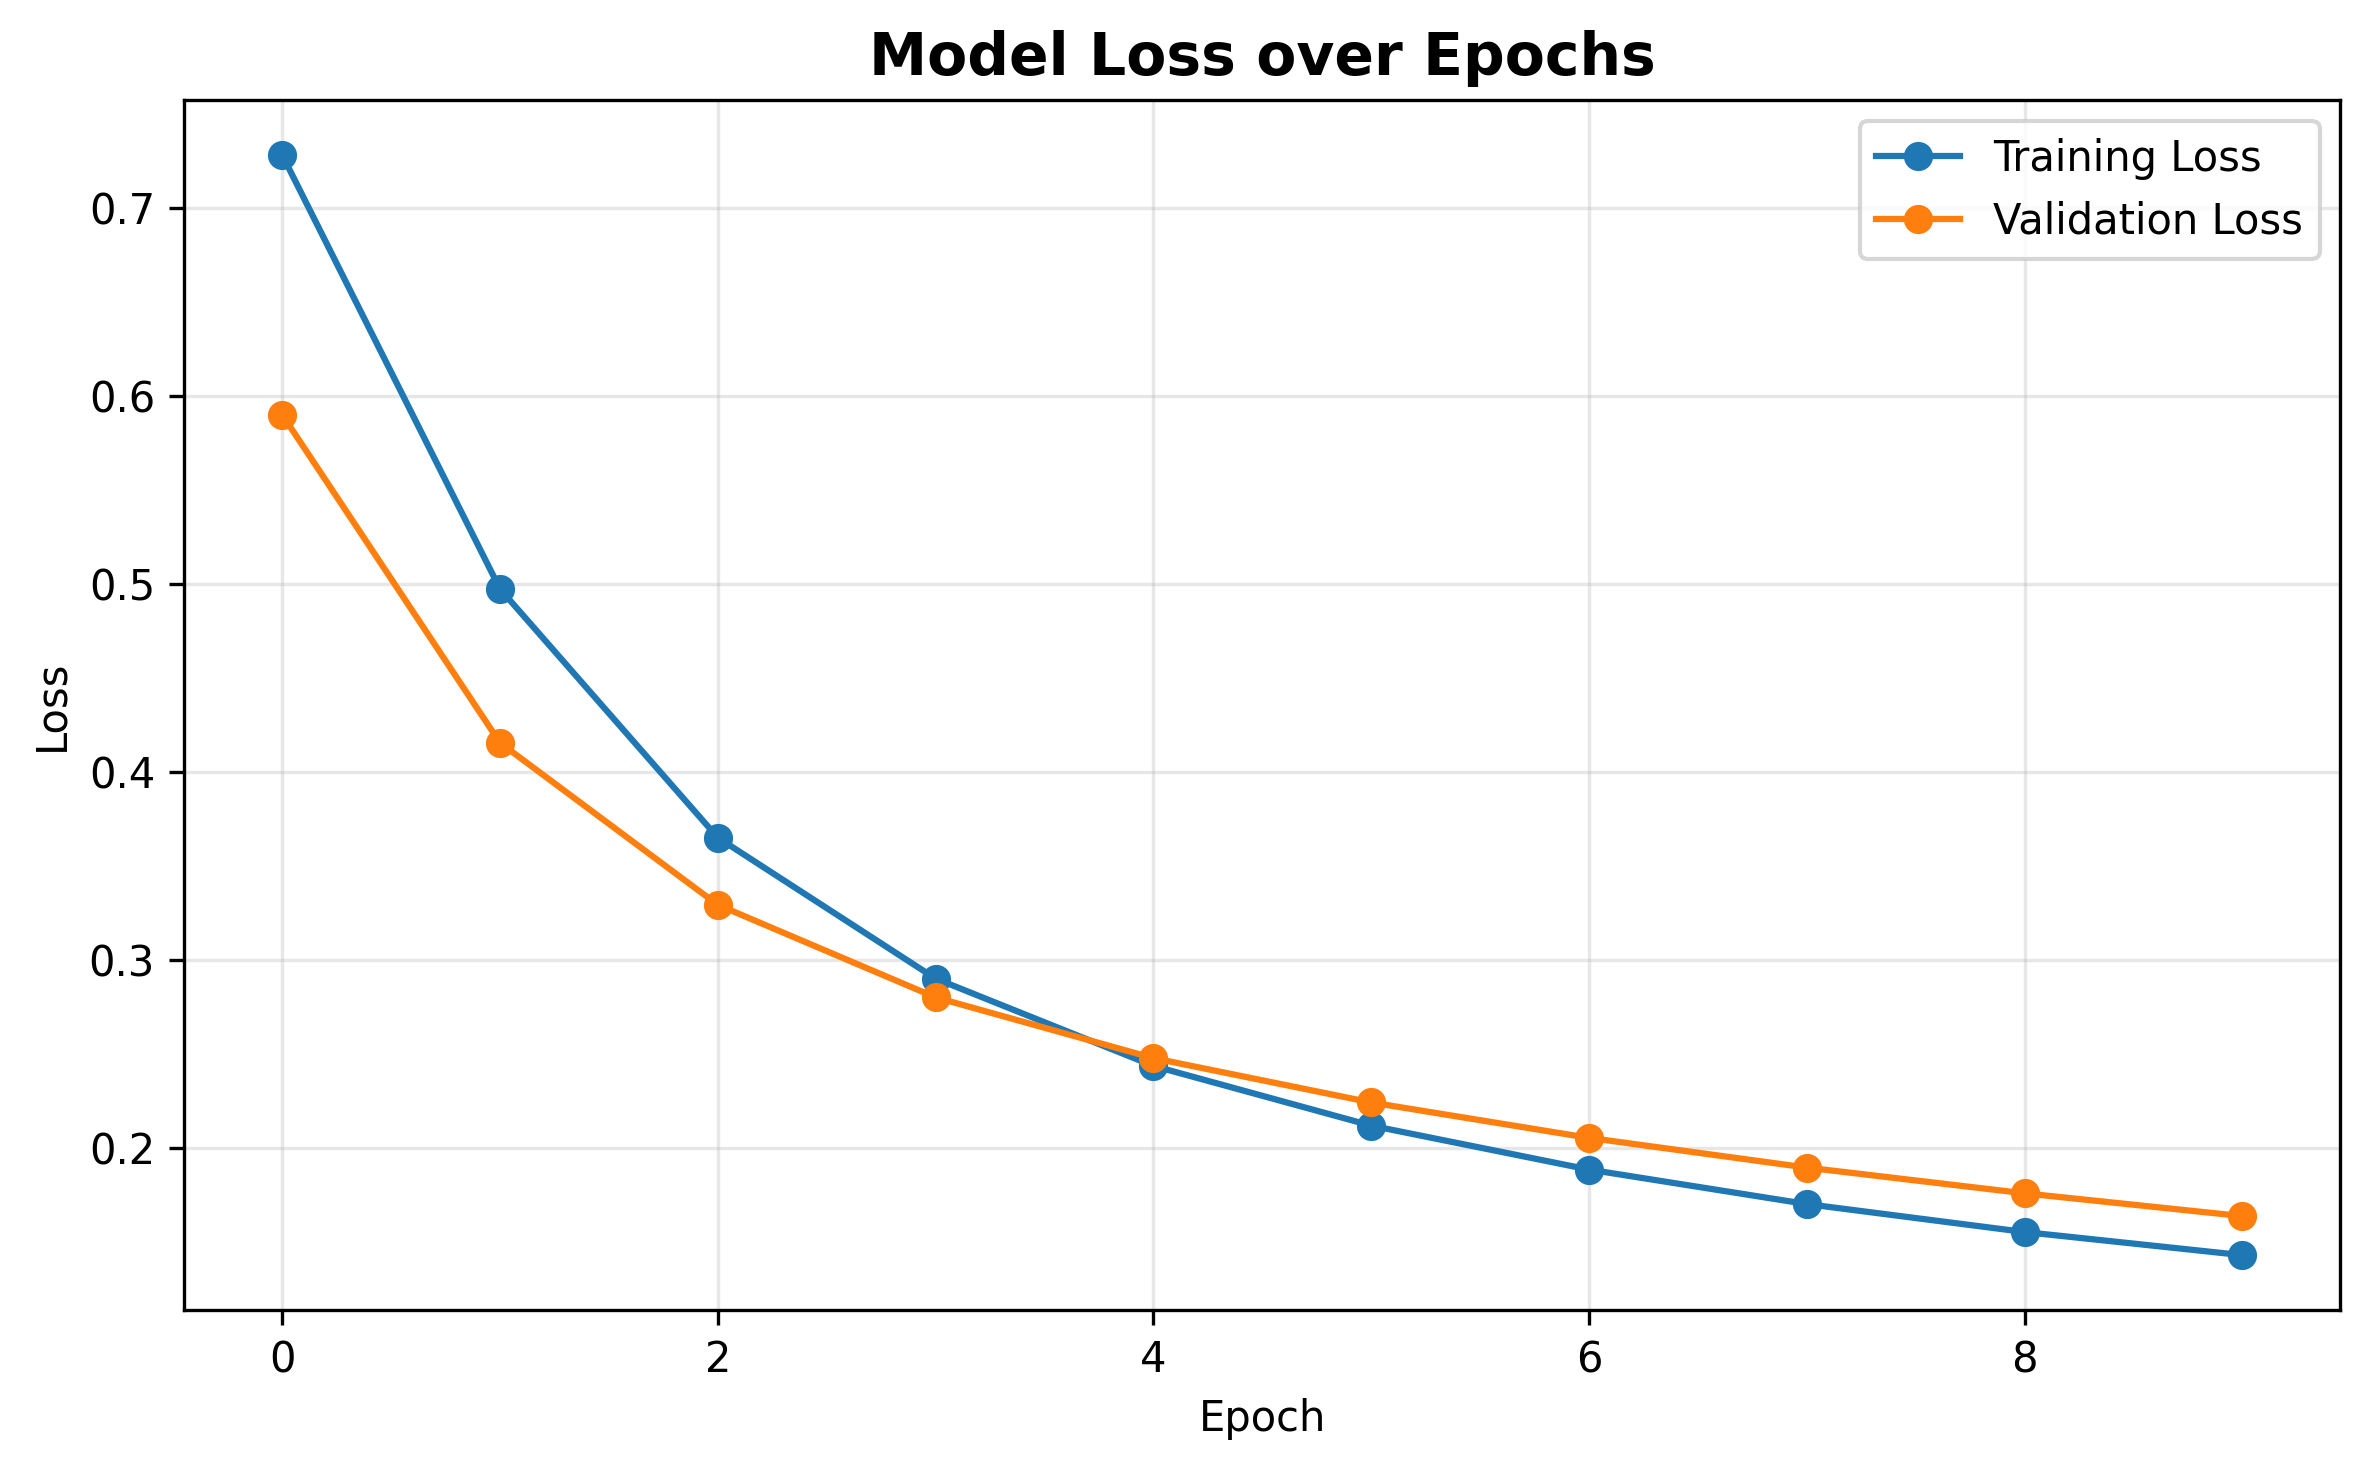
\includegraphics[width=0.85\textwidth]{06_loss_curve.png}
  \caption{Training and validation loss over epochs.}
\end{figure}

\section{Results}
\subsection{Test Performance}
\begin{figure}[H]
  \centering
  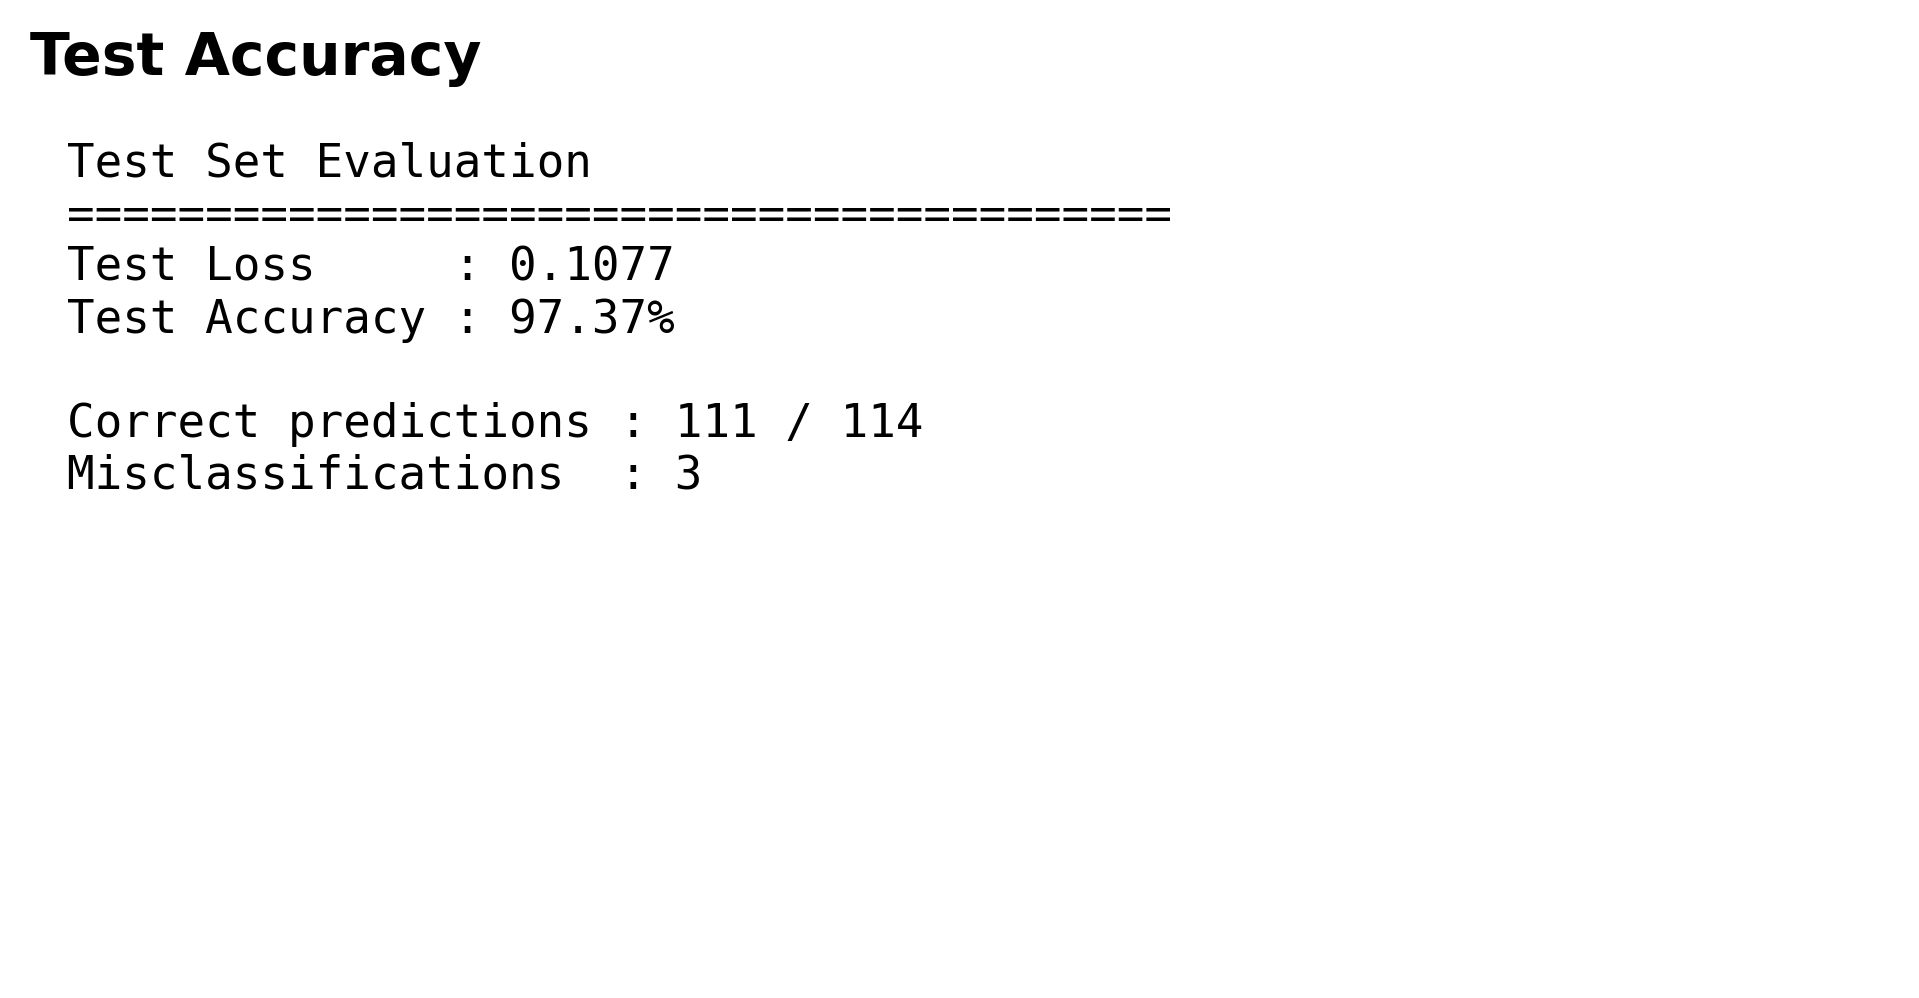
\includegraphics[width=0.8\textwidth]{07_test_accuracy.png}
  \caption{Final evaluation on the held-out test set.}
\end{figure}

\subsection{Confusion Matrix and Classification Report}
\begin{figure}[H]
  \centering
  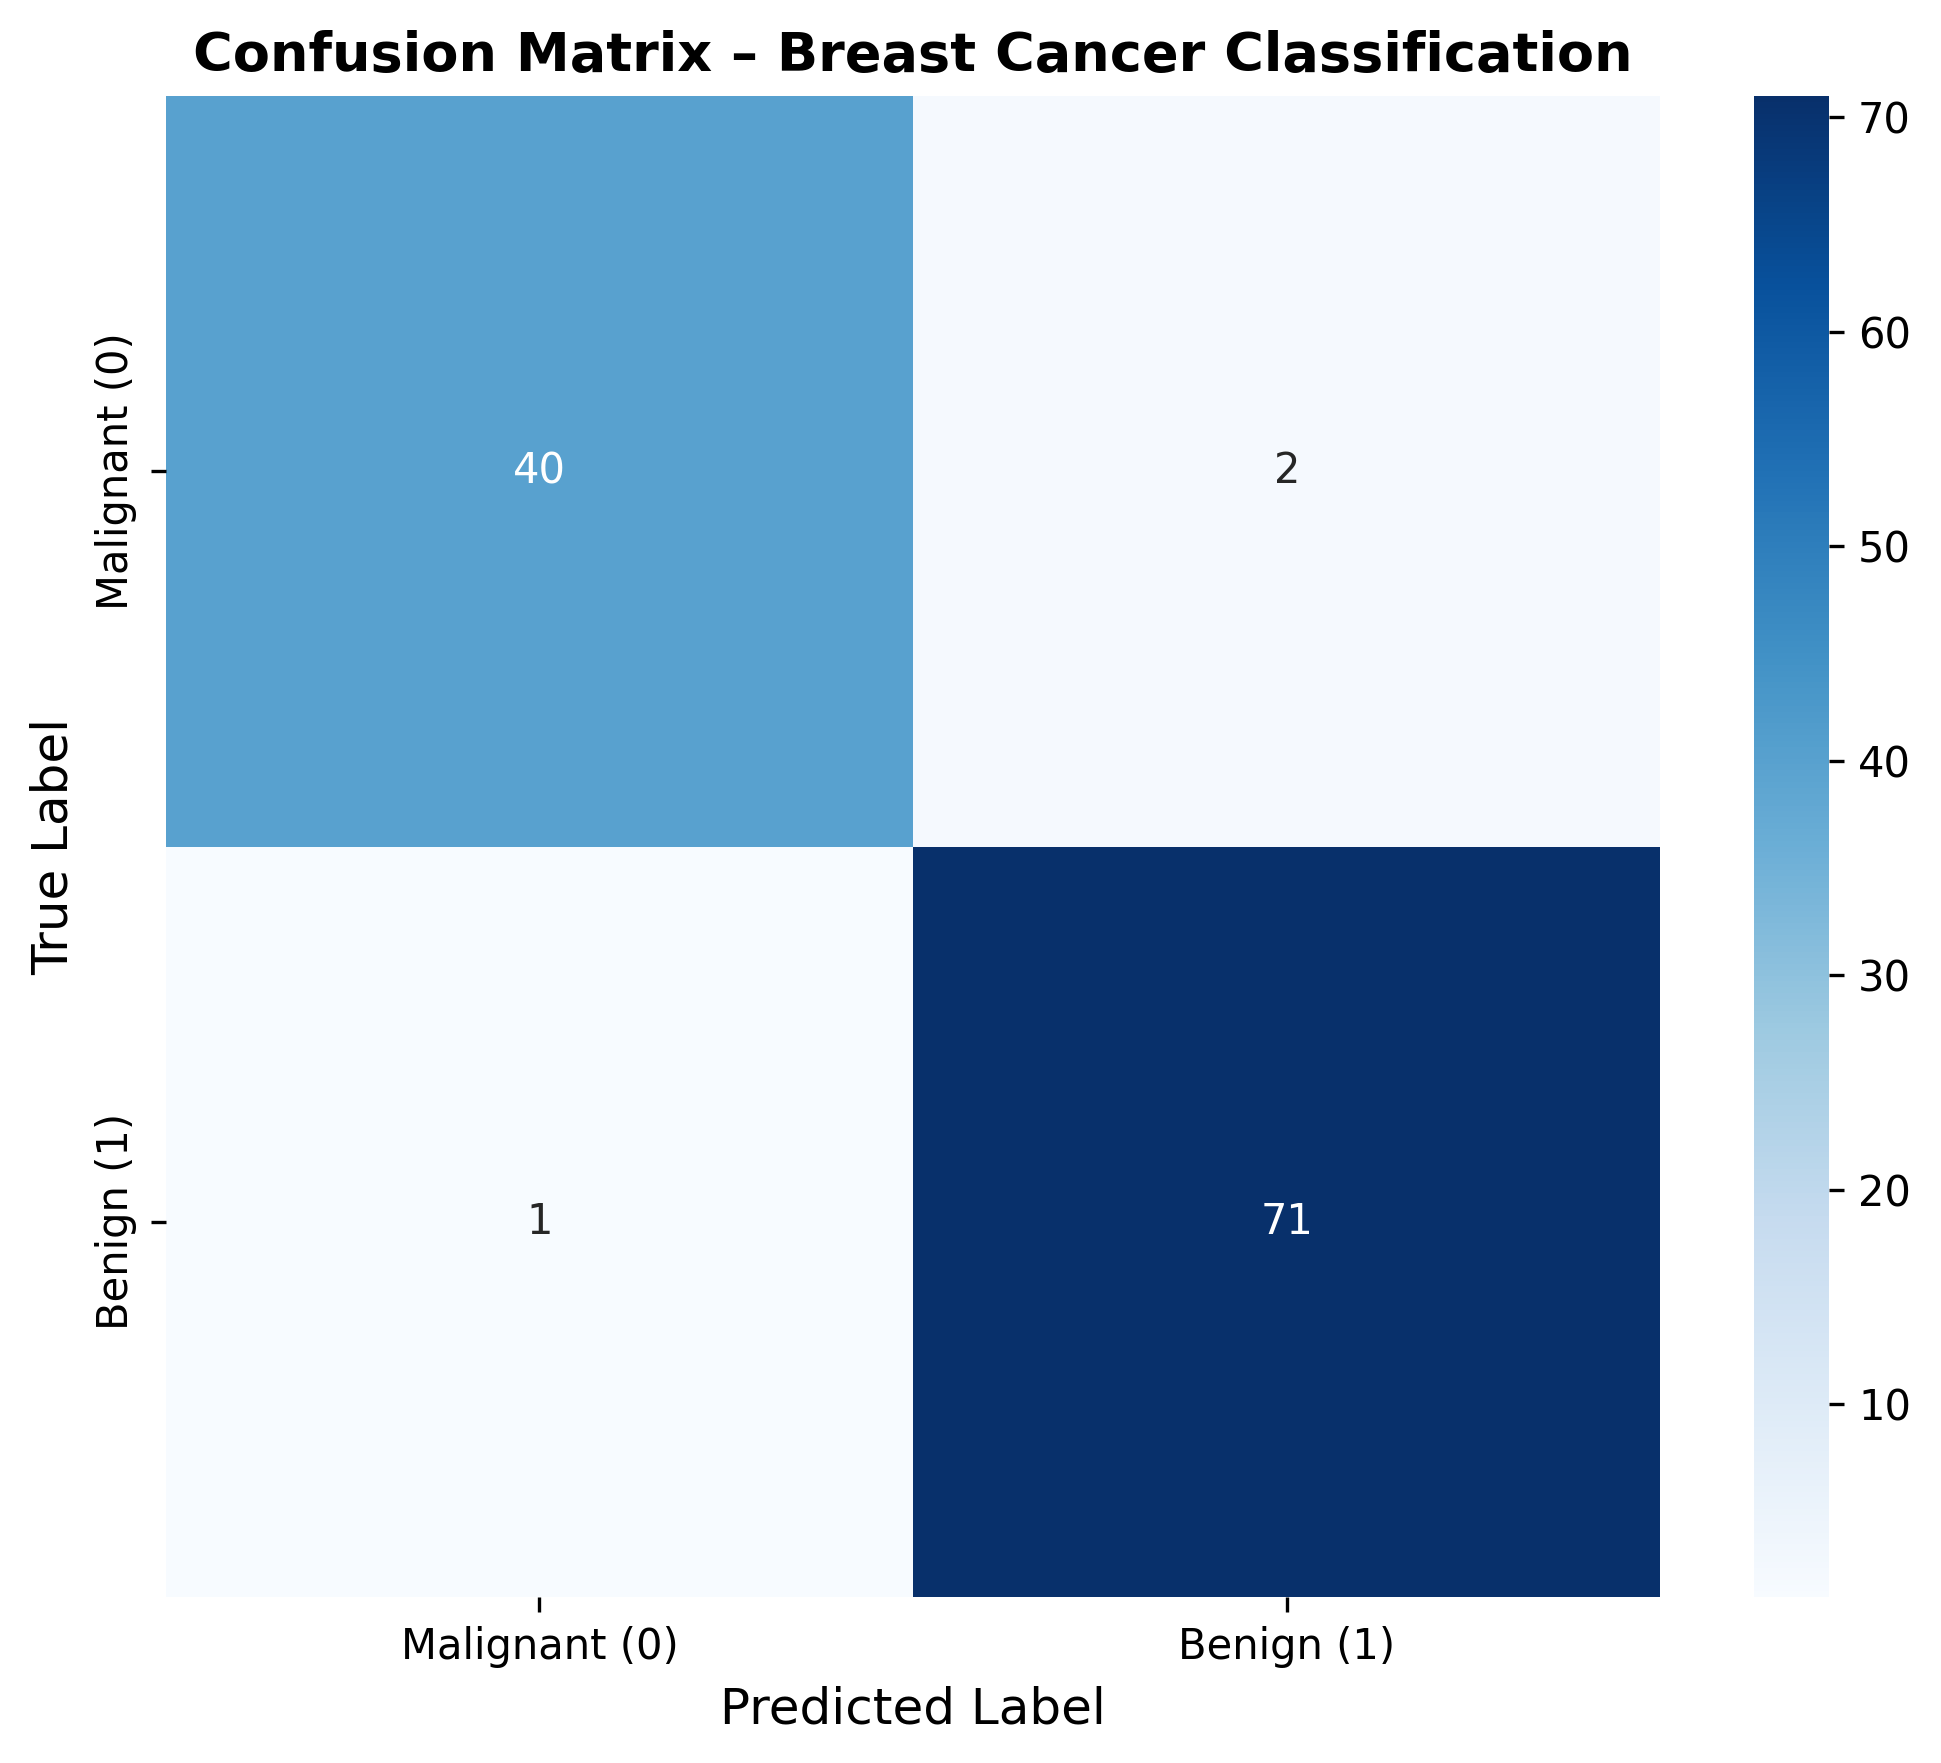
\includegraphics[width=0.75\textwidth]{08_confusion_matrix.png}
  \caption{Confusion matrix for malignant vs benign predictions.}
\end{figure}

\begin{figure}[H]
  \centering
  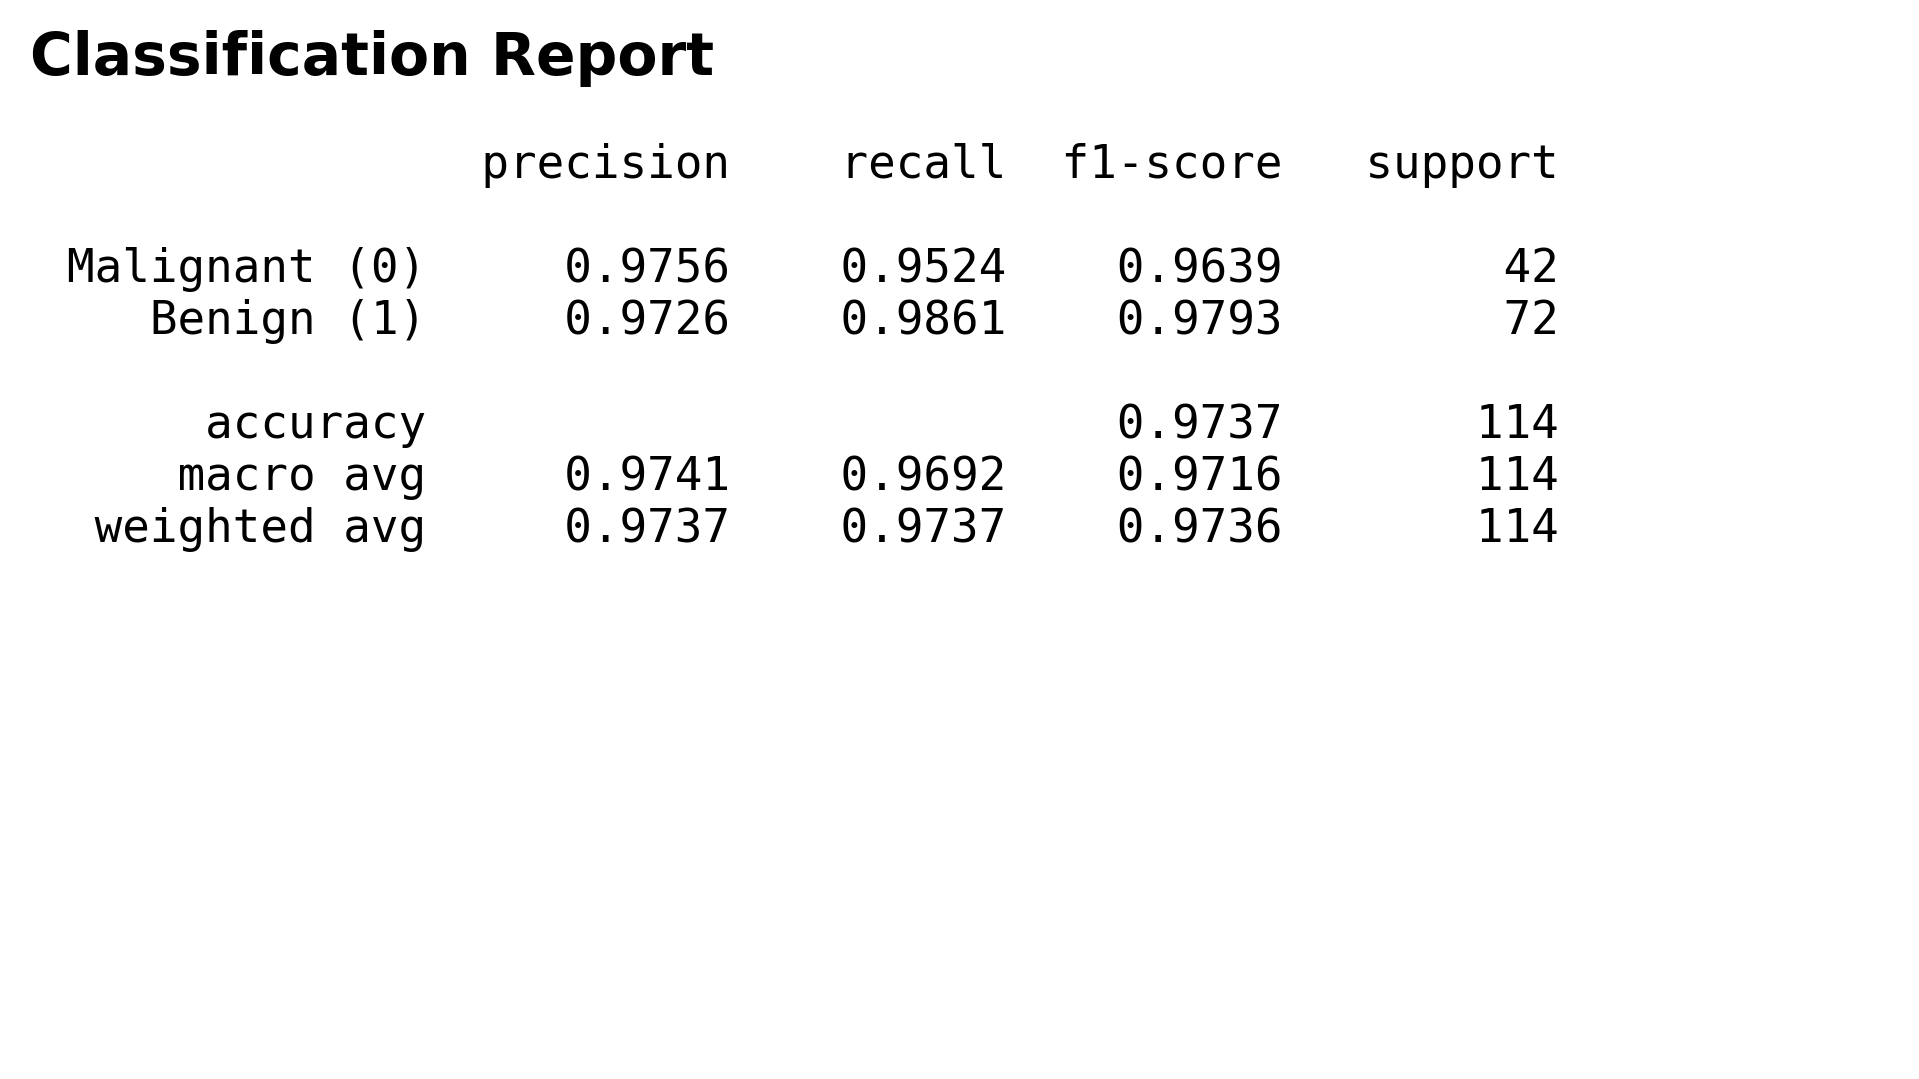
\includegraphics[width=0.9\textwidth]{09_classification_report.png}
  \caption{Precision, recall, and F1-score for each class.}
\end{figure}

\subsection{Predictive System}
A single patient sample is standardized with the fitted scaler and passed to the
trained model. The system prints the predicted diagnosis, confidence, and class
probabilities.

\begin{figure}[H]
  \centering
  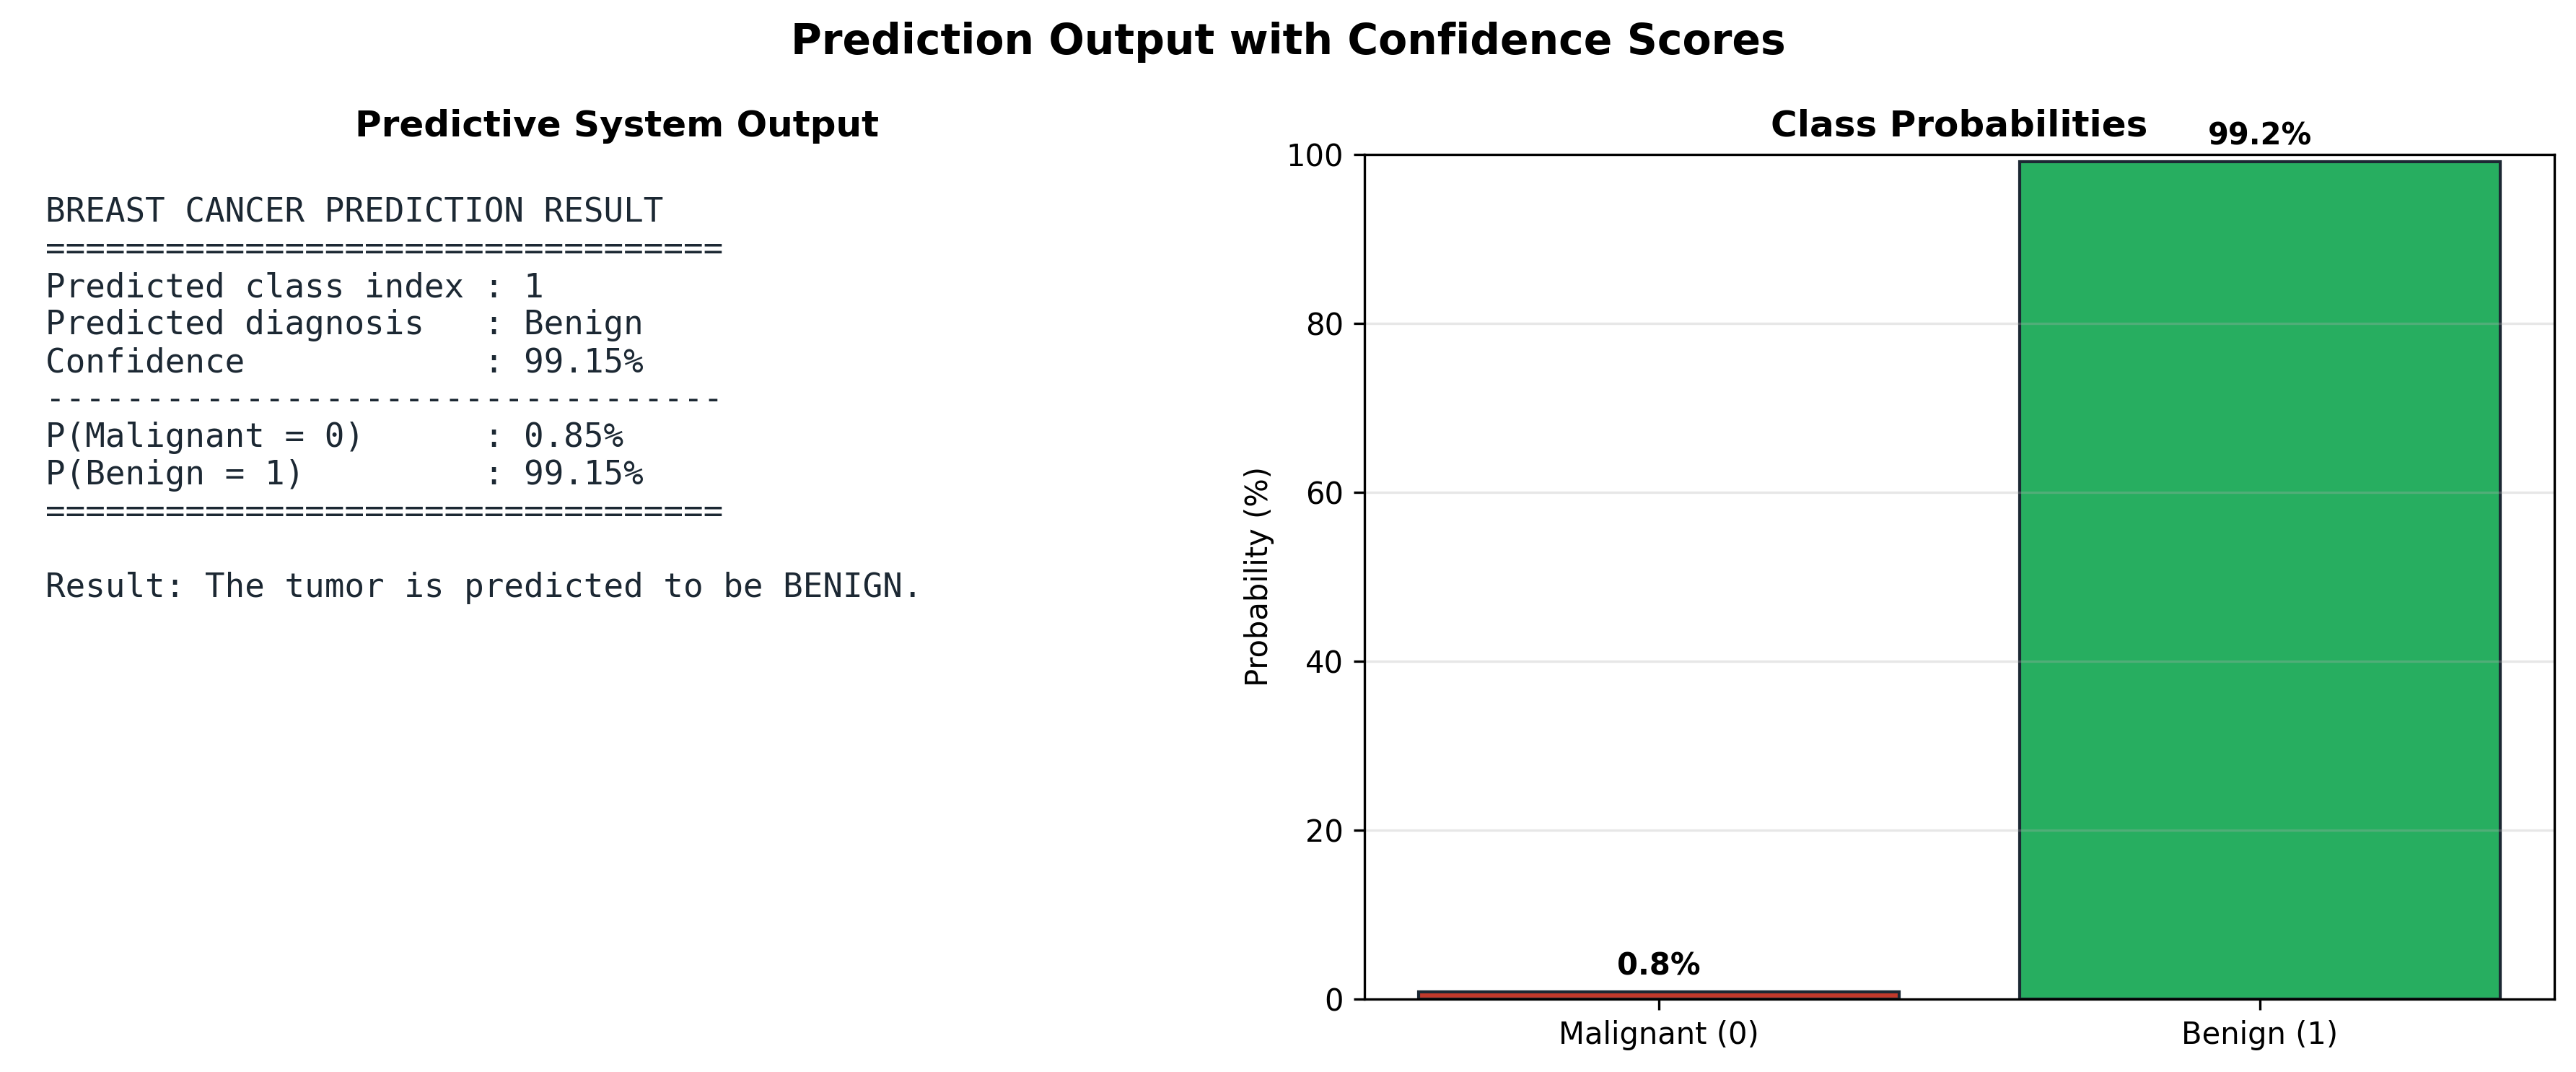
\includegraphics[width=0.95\textwidth]{10_prediction.png}
  \caption{Example prediction output with confidence scores.}
\end{figure}

\section{Project Workflow}
\begin{figure}[H]
  \centering
  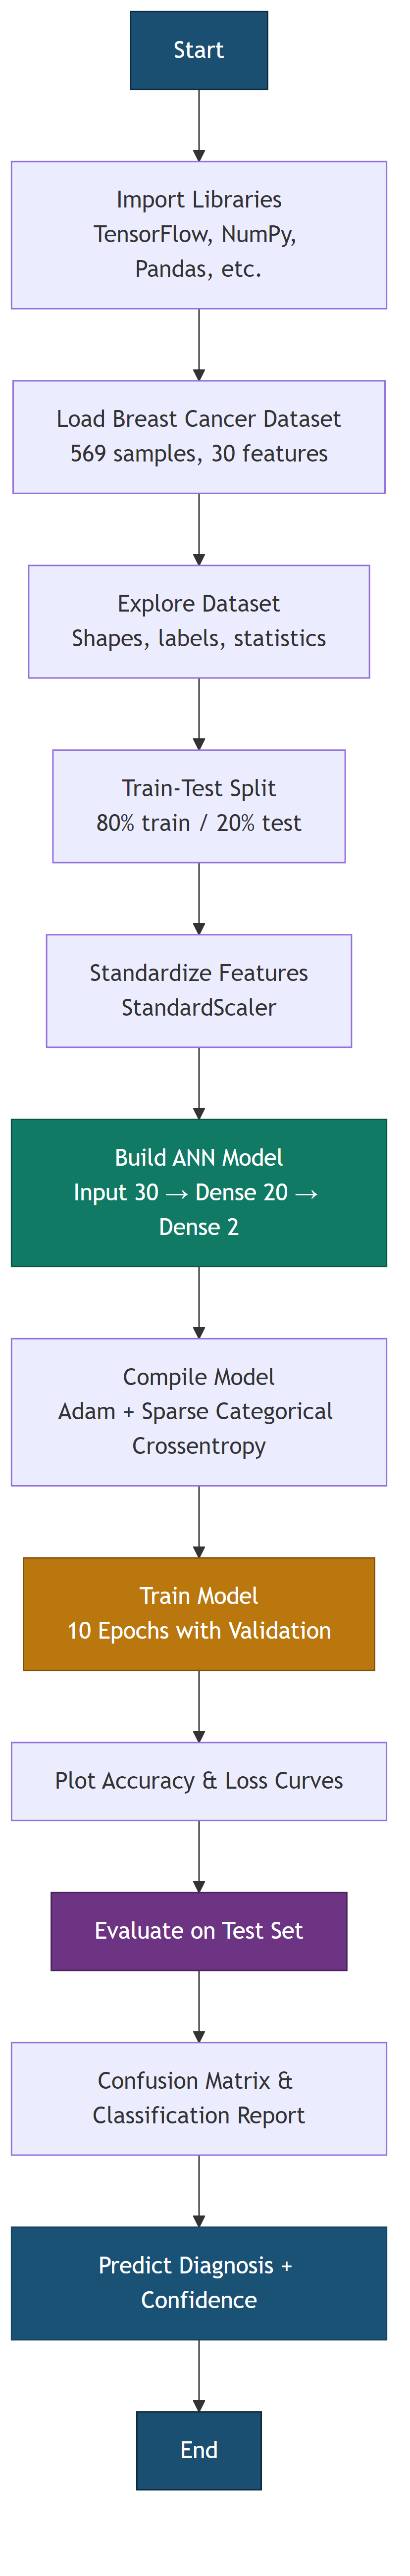
\includegraphics[width=0.55\textwidth]{11_workflow.png}
  \caption{End-to-end project workflow.}
\end{figure}

\section{Conclusion}
A simple ANN achieves strong test accuracy on the Breast Cancer Wisconsin
dataset and provides interpretable probability outputs for each diagnosis.
This pipeline demonstrates data preprocessing, neural network training,
evaluation, and a practical predictive interface suitable for academic
mini-project demonstration.

\section*{Disclaimer}
This work is for educational purposes only and is \textbf{not} a medical
diagnostic tool.

\bibliographystyle{plain}
\bibliography{references}

\end{document}
